\section{Affine Varieties}

\begin{definition}
    Let $k$ be an algebraically closed field. We define  \textbf{affine
    $n$-space} over $k$ to be the set $\A^n(k)$ of $n$-tuples of elements of
    $k$. We write simply $\A^n$ when  $k$ is understood. We call the elements of
    $\A^n$  \textbf{points} and if $P=(a_1, \dots, a_n)$ is a point of $\A^n$,
    we call each $a_i$ the \textbf{coordinates} of $P$.
\end{definition}

\begin{example}\label{example_1.1}
    Let $k$ be any algebraically closed field, and consider the multivariate
    polynomial ring $k[x_1, \dots, x_n]$. We can interperate the elements of
    $k[x_1, \dots, x_n]$ as functions from affine space $\A^n(k)$ to $k$ by
    taking  $f(P)=f(a_1, \dots, a_n)$, where $f \in k[x_1, \dots, x_n]$ and $P
    \in \A^n(k)$. This leads us to be able to talk about the set of zeros of a
    polynomial over $k$.
\end{example}

\begin{definition}
    Let $k$ be an algebraically closed field, and $f \in k[x_1, \dots, x_n]$ a
    multivariate polynomial over $k$. We define the \textbf{set of zeros} of $f$
    to be the set
    \begin{equation*}
        Z(f)=\{P \in \A^n(k) : f(P)=0\}
    \end{equation*}
    Let $T$ be a subset of  $k[x_1, \dots, x_n]$. Then we define the \textbf{set
    of zeros} of $T$ to be
    \begin{equation*}
        Z(T)=\bigcap_{f \in T}{Z(f)}
    \end{equation*}
    Now, if $\af=(f_1, \dots, f_r)$ is an ideal of  $k[x_1, \dots, x_n]$ generated
    by $T$, then we write  $Z(T)=Z(\af)=Z(f_1, \dots, f_r)$.
\end{definition}

\begin{example}\label{example_1.2}
    We have $\A^n=Z(0)$, and by convention, we also take $\A^n=Z(\emptyset)$. In
    similar fashion, we have $\emptyset=Z(1)$, and $\emptyset=Z(k[x_1, \dots,
    x_n])$.
\end{example}

\begin{definition}
    Let $k$ be an algebraically closed field. We call a subset $Y$ of $\A^n$ an
    \textbf{algebraic set} if there exists some $T \subseteq k[x_1, \dots, x_n]$
    for which $Y$ is the set of zeros of $T$; i.e. $Y=Z(T)$.
\end{definition}

\begin{lemma}\label{lemma_1.1.1}
    Let $k$ be an algebraically closed field. Then algebraic sets of $\A^n$ make
     $\A^n$ into a topology under closed sets.
\end{lemma}
\begin{proof}
    Notice that $\A^n=Z(0)$ and $\emptyset=Z(1)$. Then $\A^n$ and $\emptyset$
    are both algebraic. Now, let  $X$ and  $Y$ be algebraic, then there are $S,T$
    such that  $X=Z(S)$ and $Y=Z(T)$. Now, let $P \in X \cup Y$, then $P$ is a
    zero of any polynomial $f \in ST$, conversly, suppose that $P \in Z(ST)$ where
    $P \notin Y$. There exists a polynomial  $f \in S$ with $f(P) \neq 0$. Now,
    for any $g \in T$, we have that if $fg(P)=0$, then $g(P)=0$, so that $P \in
    S$. Therefore we have  $X \cup Y=Z(ST)$, making $X \cup Y$ algebraic. So that
    the collection of algebraic sets is closed under finite intersection.

    Lastly, consider a collection $\{Y_\alpha\}$ of algebraic sets, where
    $Y_\alpha=Z(T_\alpha)$ for some $T_\alpha$. Let
    \begin{equation*}
        Y=\bigcap{Y_\alpha} \text{ and } T=\bigcup{T_\alpha}
    \end{equation*}
    and let $P \in Y$. Then $P$ is in every $Y_\alpha$ making it a zero of some
    $f_\alpha \in T_\alpha$, thus  $P \in Z(T)$. Similarly, if $P \in Z(T)$, then
    $P \in Y$, making $Y=Z(T)$, and making the collection of algebraic sets
    closed under arbitrary intersections.
\end{proof}

\begin{definition}
    We define the \textbf{Zariski topology} on affine $n$-space  $\A^n$ to be
    the topology on $\A^n$ whose closed sets are the algebraic sets of $\A^n$.
\end{definition}

\begin{example}\label{example_1.3}
    \item[(1)] Consider the Zariski topology on affine $1$-space  $\A^1$. Now, since
        $k[x]$ is a PID,  every algebraic set of $\A^1$ is the set of zeros of
        preciesly one polynomial. Moreover, by the algebraic closure of  $k$,
        for any nonzero polynomial  $f$ over  $k$, we have
        \begin{equation*}
            f(x)=c(x-a_1) \dots (x-a_n)
        \end{equation*}
        where $c,a_1, \dots, a_n \in k$. Then $Z(f)=\{a_1, \dots, a_n\}$, so
        that the algebraic sets of $\A^1$ are the emptyset, itself, and finite
        subsets. Thus the Zariski topology on  $\A^1$ consists of finite sets,
        the emptyset, and $\A^1$ itself. Notice that this topology is not Hausdorff.

    \item[(2)] Consider the field $\C$ of complex numbers. Then the Zariski
        topology has as closed sets all algebraic sets of  $\A^n(\C)$; i.e. all
        sets of zeros of polynomials in $\C$. Now, by the fundamental theorem of
        algebra, these closed stets are finite. Consider then the polynomials
        $f(z)=z^2+1$, and $g(z)=z^3-iz^2+25z+-i25$ in $\C$. Then notice that
        $(\com{\C}{Z(f)}) \cap (\com{\C}{Z(g)})=Z(f) \cup Z(g)=\{i,-i,i25,
        -i25\}$. In general for an algebraically closed fiedl $k$, zero sets of
        polynomials over $k$ are not disjoint; so that the Zariski topology on
        $\A^n(k)$ is not Hausdorff.
\end{example}

\begin{definition}
    Let $X$ be a topological space, and  $Y$ a subspace of  $X$. We call  $Y$
     \textbf{irreducible} if it cannot be written as the union $Y=Y_1 \cup Y_2$
     of two sets $Y_1$ and $Y_2$ closed in $Y$. We make the convention that the
     emptyset is not irreducible.
\end{definition}

\begin{example}\label{example_1.4}
    \begin{enumerate}
        \item[(1)] Notice that the affine space $\A^1$ is irreducible. We have
            the only closed sets are finite sets, and since  $k$ is
            algebraically closed, and hence infinite, then  $\A^1$ must be
            infinite.

        \item[(2)] Subspaces of irreducible spaces are irreducible and dense.

        \item[(3)] If $Y$ is an irreducible space of a topological space  $X$,
            then the closure  $\cl{Y}$ is also irreducible in $X$.
    \end{enumerate}
\end{example}

\begin{definition}
    We define an \textbf{algebraic affine variety} to be an irreducible closed
    subset of $\A^1$ under the Zariski topology. We define an open set of an
    affine variety to be a  \textbf{quasi-affine variety}.
\end{definition}

\begin{definition}
    We define the \textbf{ideal} of a subset $Y$ in  $\A^n$, to be the set
    \begin{equation*}
        I(Y)=\{f \in k[x_1, \dots, x_n] : f(P)=0 \text{ for all } P \in Y\}
    \end{equation*}
    where $k$ is an algebraically closed field.
\end{definition}

\begin{theorem}[Hilbert's Nullstellensatz]\label{1.1.2}
    Let $k$ be an algebraically closed field and $\af$ an ideal of $k[x_1, \dots,
    x_n]$, and let $f \in k[x_1, \dots, x_n]$ be a polynomial vanishing at all
    points of $Z(\af)$. Then there exists an $r \in \Z^+$ for which  $f^r \in
    \af$.
\end{theorem}

\begin{lemma}\label{1.1.3}
    The followin are true for any algebraically closed field $k$.
    \begin{enumerate}
        \item[(1)] If $T_1,T_2 \subseteq k[x_1, \dots, x_n]$ with $T_1 \subseteq
            T_2$, then $Z(T_2) \substeq Z(T_2)$.

        \item[(2)] If $Y_1,Y_2 \subseteq \A^n$ with $Y_1 \subseteq Y_2$, then
            $I(Y_2) \subseteq I(Y_1)$.

        \item[(3)] For any $Y_1, Y_2 \subseteq \A^n$, $I(Y_1 \cup Y_2)=I(Y_1)
            \cap I(Y_2)$.

        \item[(4)] For any ideal $\af$ of  $k[x_1, \dots, x_n]$,
            $I(Z(J))=\sqrt{\af}$, where
            \begin{equation*}
                \sqrt{\af}=\{f \in k[x_1, \dots, x_n] : f^r \in J \text{ for
                    some } r \in \Z^+\}
            \end{equation*}

        \item[(5)] For every $Y \subseteq \A^n$,  $Z(I(Y))=\cl{Y}$ in the
            Zariski topology.
    \end{enumerate}
\end{lemma}
\begin{proof}
    Let $T_1 \subseteq T_2$ be subsets of $k[x_1, \dots, x_n]$, and choose a
    polynomial $f \in T_1$, and a point $P \in Z(T_2)$. We have by inclusion
    that $f \in T_2$, and that $f(P)=0$. Now since $f \in T_1$, this puts $P \in
    Z(T_1)$ and we get the required inclusion. The proof for statement (2) is
    identical.

    Now, let $P \in Y_1 \cup Y_2$, and choose a polynomial $f \in I(Y_1) \cap
    I(Y_2)$. Then we have that the point $P$ is either contained in  $Y_1$ or
    $Y_2$ (or both), so that $f(P)=0$, which makes $I(Y_1 \cup Y_2) \subseteq
    I(Y_1) \cap I(Y_2)$. Conversely, if $f \in I(Y_1) \cap I(Y_2)$, then for any
    points $P \in Y_1 \cup Y_2$, $f(P)=0$, which puts $f \in I(Y_1 \cup Y_2)$.

    For part (4), notice this is a direct consequence of Hilbert's
    Nullstellensatz. Now, for part (5), notice that $Y \subseteq Z(I(Y))$, which
    is a closed set in the Zariski topology, so that $\cl{Y} \subseteq Z(I(Y))$.
    Now, let $W$ be a closed set in  $\A^n$, containing $Y$. Then we have
    $W=Z(\af)$, for some ideal $af$ of  $k[x_1, \dots, x_n]$, so that $Y \subseteq
    Z(\af)$. Then by part (2), observe that $I(Y) \subseteq I(Z(\af))$, but $\af
    \subseteq I(Z(\af))$, so by part (1), we have $Z(I(Y)) \subseteq Z(\af)$. This
    makes $Z(I(Y))=\cl{Y}$.
\end{proof}
\begin{corollary}
    There exists a 1--1, inclusion reversing, corresponedece of algebraic sets
    of $\A^n$ onto radical ideals in $k[x_1, \dots, x_n]$; given by the maps
    \begin{equation*}
        \begin{array}{lcl}
            Y   &   \xrightarrow{}  &   I(Y)    \\
            \af   &   \xrightarrow{}  &   Z(\af)    \\
        \end{array}
    \end{equation*}
    Moreover, an algebraic set in $\A^n$ is irreducible if, and only if its
    ideal in $k[x_1, \dots, x_n]$ is prime.
\end{corollary}
\begin{proof}
    Notice that parts (1), (2), and (3) of the above lemma provide the required
    correspondence.

    Now, suppose that $Y$ is irreducible in  $\A^n$, and take  $fg \in I(Y)$.
    Then $Y \subseteq Z(fg)=Z(f) \cup Z(g)$, so that
    \begin{equation*}
        Y=(Y \cap Z(f)) \cup (Y \cap Z(g))
    \end{equation*}
    which is the union of two closed sets in $\A^n$. Now, since $Y$ is
    irreducible, we get that either  $Y=Y \cap Z(f)$, or $Y=Y \cap Z(g)$; in
    either case, $Y \subseteq Z(f)$, or $Y \subseteq Z(g)$. This puts either $f
    \in I(Y)$, or $g \in I(Y)$, which makes the ideal $I(Y)$ prime.

    Conversely if $\pf$ is a prime ideal, let  $Z(\pf)=Y_1 \cup Y_2$, then
    $\pf=I(Y_1) \cap I(Y_2)$, so that either $\pf=I(Y_1)$ or $\pf=I(Y_2)$,
    since $\pf$ is prime. This makes  $Z(\pf)=Y_1$ or $Z(\pf)=Y_2$,  which makes
    $Z(\pf)$ irreducible in $\A^n$.
\end{proof}

\begin{example}\label{example_1.5}
    Consider $k$ to be an algebraically closed field.
    \begin{enumerate}
        \item[(1)] Notice that $\A^n$ maps to the ideal $(0)$ in $k[x_1, \dots,
            x_n]$, which is a prime ideal. This makes $\A^n$ irreducible by
            the corollary to lemma \ref{1.1.3}.

        \item[(2)] Let $f \in k[x,y]$ be an irreducible polynomial. Then $f$
            generates the prime ideal  $(f)$ in $k[x,y]$, since $k[x,y]$ is a
            UFD. Thus the zero set $Y=Z(f)$ is irreducible, and closed in
            $\A^n$; hence it is an affine variety. We call $Y$ an
            \textbf{affine curve} in $\A^n$ defined by the equation $f(x,y)=0$
            of \textbf{degree} $\deg{f}=d$. Now, moregenerally, if $f$ is an
            irreducible polynomial in $k[x_1, \dots, x_n]$, then we call the
            affine variety $Y=Z(f)$ a \textbf{surface} in $n=3$ and a
            \textbf{hypersurface} in $n>3$.

        \item[(3)] A maximal ideal $\mf$ of $k[x_1, \dots, x_n]$ correspondes to
            a minimal affine variety of $\A^n$, which are the point-sets $\{P\}$
            of $\A^n$; where  $P=(a_1, \dots, a_n)$. Thus every maximal ideal of
            $k[x_1, \dots, x_n]$ is of the form $M=(x_1-a_1, \dots,x_n-a_n)$ for
            some $a_1, \dots, a_n \in k$.

        \item[(4)] Consider the field $\R$ which is not algebraically closed, and
            the curve defined by $x^2+y^2+1=0$ in $\A^2(\R)$. Notice that this
            curve is irreducible, but has no points in $\A^2$  (i.e. no roots
            in $\R$). This shows that if the field $k$ is no algebraically
            closed, then the above results do not hold in general. Notice that
            the paraboloid $f(x,y)=x^2+y^2+1$ (figure \ref{figure_1.1}) does not
            intersect the real $xy$-plane
             \begin{figure}[h]
                \centering
                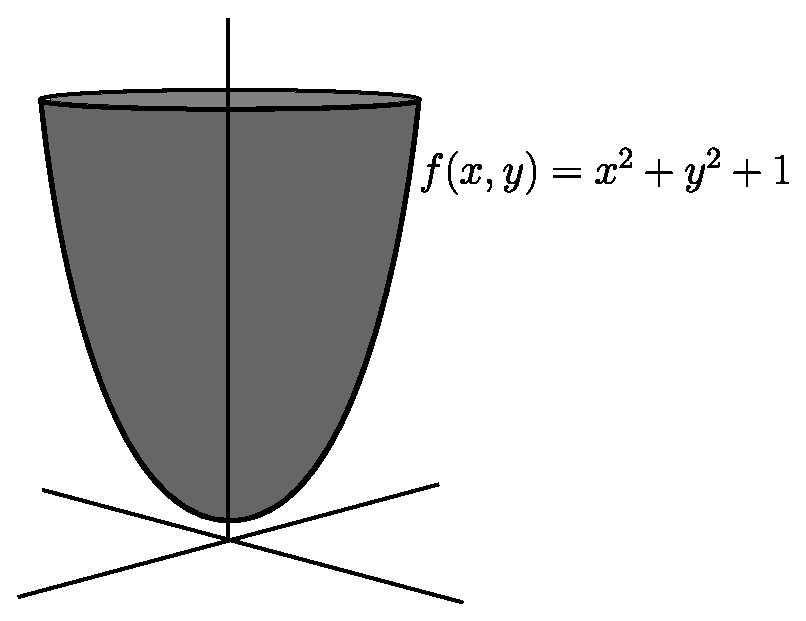
\includegraphics[scale=0.7]{Figures/chapter1/non_affine_variety.eps}
                \caption{The curve $x^2+y^2+1=0$ does not describe an affine
                variety.}
                \label{figure_1.1}
            \end{figure}
    \end{enumerate}
\end{example}

\begin{definition}
    Let $k$ be an algebraically closed field, and $Y$ an affine algebraic set of
     $\A^n$. We definen the \textbf{affine coordinate ring} of $Y$ to be the
     factor ring
     \begin{equation*}
         A(Y)=\faktor{k[x_1, \dots, x_n]}{I(Y)}
     \end{equation*}
\end{definition}

\begin{lemma}\label{1.1.4}
    If $Y$ is an affine variety, then  $A(Y)$ is an integral domain. Moreover,
    there exists a 1--1 correspondence of finitely generated $k$-algebras onto
    affine coordinate rings of affine varieties.
\end{lemma}

\begin{definition}
    We call a topological space X \textbf{Noetherian} if it satisfies
    the descending chain condition on closed sets; that is, if
    \begin{equation*}
        \dots \subseteq Y_2 \subseteq Y_1
    \end{equation*}
    is a descending chain of closed sets in $X$, then there exists an  $r \in
    \Z^+$ for which  $Y_r=Y_{r+1}=\dots$
\end{definition}

\begin{example}\label{example_1.6}
    Let $\dots \subseteq Y_2 \subseteq Y_1$ be a descending chain of closed sets
    in $\A^n$. Then  $I(Y_1) \subseteq I(Y_2) \subseteq \dots$ is an ascending
    chain of ideals of $k[x_1, \dots, x_n]$. Since $k[x_1, \dots, x_n]$ is
    Noetheria, we get an $r \in \Z^+$ for which  $I(Y_r)=I(Y_{r+1})=\dots$.
    Since $Y_r=Z(I(Y_r))$, this makes $Y_r=Y_{r+1}=\dots$. This makes $\A^n$ a
    Noetherian space.
\end{example}

\begin{lemma}\label{lemma_1.1.5}
    If $X$ is a Noetherian space, then every nonempty closed set  $Y$ in  $X$
    can be written as a finite union of irreducible closed sets of  $X$; i.e.
    \begin{equation*}
        Y=\bigcup_{i=1}^r{Y_i}
    \end{equation*}
    where each $Y_i$ is closed and irreducible in $X$. Moreover, if $Y_i
    \not\subseteq Y_j$ for all  $i \neq j$, then this representation is unique.
\end{lemma}
\begin{proof}
    Let $\Cc$ be the collections of nonempty closed sets in  $X$, which are not
    expressable as a finite union of closed irreducible sets in  $X$. Suppose
    that $\Cc$ is nonempty. Since $X$ is Noetherian, $\Cc$ contains a minimal
    elements $Y$. Then by definition, we have $Y=Y_1 \cup Y_2$ where $Y_1$ and
    $Y_2$ are closed sets; and by the minimality of $Y$, they can be expressed
    as a finite union of closed irreducible sets in $X$. This makes $Y$ a finite
    union of closed irreducible sets of  $X$, which means  $Y \notin \Cc$; a
    contradiction of our assumption that  $Y$ is the minimal element. Therefore
     $\Cc$ must be empty, and every closed set  $Y$ is the finite union of
     closed irreducible sets in  $X$.

     Now, let  $Y=\bigcup_{i=1}^r{Y_i}$ where each $Y_i$ is closed and
     irreducible in  $X$; and suppose that for each  $i \neq j$,  $Y_i
     \notsubseteq Y_j$. Let
     \begin{equation*}
         Y=\bigcup_{j=1}^s{Z_j}
     \end{equation*}
     another representation of $Y$ as a finite union of closed irreducible sets
     in  $X$. Notice that that  $Z_1 \subseteq Y_1 \cup \dots Y_r$, so that
     \begin{equation*}
         Z_1=\bigcup_{i=1}^r{(Z_1 \cap Y_i)}
     \end{equation*}
     since $Z_1$ is irreducible, we get $Z_1 \subseteq Y_i$ for some $i$, and
     $Y_1 \subseteq Z_j$ for some $j$. This gives that $Y_1=Z_j$. Now, let
     $Z=(\com{Y}{Y_1})^-$ then $Z=Y_2 \cup \dots \cup Y_r$, and $Z=Z_2 \cup
     \dots \cup Z^s$. Proceeding inductively gives us the desired uniqueness.
\end{proof}
\begin{corollary}
    Every affine algebraic set in $\A^n$ can be uniquely expressed as a finite
    union of affine varieties, no one containing the other.
\end{corollary}

\begin{definition}
    We define the \textbf{dimension} of a topological space $X$ to be the
    suprememum on all integers  $n \geq 0$ for which there is a chain
    \begin{equation*}
        Z_0 \subseteq \dots \subseteq Z_n
    \end{equation*}
    of distinct irreducible closed sets in $X$, we write  $\dim{X}=n$.
\end{definition}

\begin{example}\label{example_1.7}
    The dimension of $\A^1$ under the Zariski topology is  $\dim{\A^1}=1$, since
    the only irreducible closed sets are $\A^1$ and point-sets.
\end{example}

\begin{definition}
    Let $A$ be a ring. We define the  \textbf{height} of a prime ideal $\pf$ to
    be the suprememum on all integeres  $n \geq 0$ for which there exists a
    chain
    \begin{equation*}
        \pf_0 \subseteq \dots \pf_n=\pf
    \end{equation*}
    of distinct prime ideals, and write $\height{\pf}=n$. We define the
    \textbf{Krull-dimension}of $A$ to be
    \begin{equation*}
        \dim{A}=\sup_{\pf \subseteq A}{\{\height{\pf}\}}
    \end{equation*}
    where the suprememum is taken over all prime ideals of $A$.
\end{definition}

\begin{lemma}\label{1.1.6}
    If $Y$ is an affine algebraic set, then  $\dim{Y}=\dim{A(Y)}$; that is, the
    dimension of $Y$ is the dimension of the affine coordinate ring of  $Y$.
\end{lemma}
\begin{proof}
    SUppose that $Y$ is an affine algebraic set in  $\A^n$, then the affine
    varieties of  $Y$ correspond to the prime ideals of  $k[x_1, \dots, x_n]$
    containing $I(Y)$. This in turn correspond to the prime ideals of $A(Y)$.
    Hence $\dim{Y}$ is the length of the longest chain of prime ideals in
    $A(Y)$, which is $\dim{A(Y)}$ by definition of the Krull-dimension.
\end{proof}

\begin{theorem}\label{1.1.7}
    Let $k$ be a field and  $B$ an integral domain which is a finitely generated
     $k$-algebra. Then the following are true
     \begin{enumerate}
         \item[(1)] $\dim{B}$ is the transcendence degree of the factor field
             $K(B)$ of $B$ over  $k$.

         \item[(2)] For every prime ideal $\pf$ in  $B$
             \begin{equation*}
                 \height{\pf}+\dim{\faktor{B}{\pf}}=\dim{B}
             \end{equation*}
     \end{enumerate}
\end{theorem}

\begin{lemma}\label{1.1.8}
    $\dim{\A^n}=n$.
\end{lemma}
\begin{proof}
    We have that $A(\A^n)$ is an integral domnain, so by theorem \ref{1.1.7}, the
    transcendence degree of $K(\A^n)$ of $\A^n$ over $k$ is $n$, so that
    $\dim{\A^n}=\dim{A(\A^n)}=n$.
\end{proof}

\begin{lemma}\label{1.1.9}
    If $Y$ is a quasi-affinee varaiety, then  $\dim{Y=\dim{(\cl{Y})}}$.
\end{lemma}
\begin{proof}
    Let $Z_0 \subseteq \subseteq Z_n$ be a chain of distinct closed irreducible
    sets of $Y$. Then  $\cl{Z_0} \subseteq \dots \subseteq \cl{Z_n}$ is a chain
    of closed irreducible sets in $\cl{Y}$ (not necessarily distinct), so that
    $\dim{Y} \leq \dim{(\cl{Y})}$.

    Now, $\dim{Y}$ is finite, so choose a maximal chain $Z_0 \subseteq \dots
    \subseteq Z_n$ for which $\dim{Y}=n$. Then $Z_0$ must be a point and
    $P:\cl{Z_0} \subseteq \dots \subseteq \cl{Z_n}$ is also a maximal chain. Now,
    this maximal chain corresponds to a maximal ideal $\mf$ of the affine
    coordinate ring  $A(\cl{Y})$ of $\cl{Y}$. Then $\cl{Z_i}$ corresponds to a
    prime ideal in $\mf$, so that  $\height{\mf}=n$. Now, we have that $P$ is a
    point in affine space, and since
    \begin{equation*}
        \faktor{A(\cl{Y})}{\mf} \simeq k
    \end{equation*}
    we get $n=\dim{A(\cl{Y})}=\dim{(\cl{Y})}$, so that $\dim{Y}=\dim{(\cl{Y})}$.
\end{proof}

\begin{theorem}[Krull's Hauptidealsatz]\label{1.1.10}
    Let $A$ be a Noetherian ring and $f \in A$ be an element which is neither a
    unit, nor a zero divisor. Then every minimal prime ideal $\pf$ containing
    $f$ has $\height{\pf}=1$.
\end{theorem}

\begin{lemma}\label{1.1.11}
    A Noetherian integral domain is a unique factorization domain if, and only
    if every prime ideal of  $\height=1$ is a principle ideal.
\end{lemma}

\begin{lemma}\label{1.1.12}
    An affine variety $Y$ of  $\A^n$ has dimension $n-1$ if and only if it is
    the zero set $Z(f)$ of a single irreducible polynomial $f \in k[x_1, \dots,
    x_n]$.
\end{lemma}
\begin{proof}
    Notice that if $f \in k[x_1, \dots, x_n]$ is irreducible, then the set
    $Y=Z(f)$ is an affine variety and its ideal is the prime ideal $(f)$ of
    height $1$. Hence, by theorem \ref{1.1.7} we have
    \begin{equation*}
        \dim{Y}=n-1
    \end{equation*}

    Conversely, if $Y$ is an affine variety of dimension  $n-1$, it corresponds
    to an ideal of height $1$. Now, we have that $k[x_1, \dots, x_n]$ is a UFD,
    so this prime ideal is a principle ideal and generated by a nonconstant
    polynomial $f$. This makes  $Y=Z(f)$.
\end{proof}
